\documentclass[10pt, a4paper]{article}
\usepackage{lrec2014}
\usepackage{graphicx}
\usepackage{url}
\usepackage[hidelinks]{hyperref}
\usepackage[utf8]{inputenc}
\interfootnotelinepenalty=10000

\title{Guampa: a Toolkit for Collaborative Translation}

\name{Alex Rudnick$^1$, Taylor Skidmore$^1$, Alberto Samaniego$^2$, Michael Gasser$^1$}

\address{$^1$ School of Informatics and Computing, Indiana University \\
         $^2$ Universidad Católica ``Nuestra Señora de la Asunción" \\
         \{alexr,taylskid,gasser\}@indiana.edu, alberto\_samaniego@uca.edu.py \\}

\abstract{
Here we present Guampa, a new software package for online
collaborative translation. This system grows out of our discussions with
Guarani-language activists and educators in Paraguay, and attempts to address
problems faced by machine translation researchers and by members of any
community speaking an under-represented language. Guampa enables volunteers and
students to work together to translate documents into heritage languages, both
to make more materials available in those languages, and also to generate
bitext suitable for training machine translation systems.
While many approaches to crowdsourcing bitext corpora focus on Mechanical Turk
and temporarily engaging anonymous workers, Guampa is intended to foster an
online community in which discussions can take place, language learners can
practice their translation skills, and complete documents can be translated.
This approach is appropriate for the Spanish-Guarani language pair as there are
many speakers of both languages, and Guarani has a dedicated activist
community.
Our goal is to make it easy for anyone to set up their own instance of Guampa
and populate it with documents -- such as automatically imported Wikipedia
articles -- to be translated for their particular language pair. Guampa is
freely available and relatively easy to use. \\ \newline
\Keywords{under-resourced languages, collaboration, translation, language
resources, open source}}


\begin{document}

\maketitleabstract

\section{Introduction}
For most of the world's language pairs, large bitext corpora are not readily
available and would be difficult to construct. However, for some language
pairs, not only are there many speakers of both languages, there is a community
of activists dedicated to the continued vitality of their heritage language. In
many of these cases, these speaker/activists recognize that there is a shortage
of written material in their heritage language and that translation from other
languages can help to address this problem. Thus they are often aware of the
contribution that machine translation (MT) would make to their task and are eager to do their part in
creating the bitext corpora that are required for statistical MT (SMT). At the same time, they
know that in the absence of MT systems, it is up to the bilingual speakers
themselves to perform the required translations. This is a daunting task for a
small community, however, and collaborative translation can speed up the
process.

In such contexts it thus makes sense to consider a tool that would facilitate
collaborative translation as well as the gathering of translation examples for
a corpus. We know of no user-friendly FOSS software for collaboratively
translating documents on the web, at least not with an eye towards training MT
systems. We address this perceived need with Guampa, a free software package
for the online collaborative translation of documents. It is meant to help both
language activist/learner communities in generating resources for their
heritage languages and MT researchers in building bitext corpora. We are
especially interested in the common case of language pairs in which one
language (normally the source for translation) has substantial resources but
the other (normally the target) does not. Guampa includes tools for importing
source language articles from Wikipedia as well as exporting bitext suitable
for training MT systems.

\section{Spanish and Guarani in Paraguay}
Our group is particularly interested in building a larger bitext corpus for the
Spanish-Guarani language pair. Spanish and Guarani are the co-official
languages of Paraguay, where most people speak Guarani as their first language
and many are bilingual. Guarani suffers not only from a serious lack of
written materials but also from a neglect in many aspects of public life in
Paraguay. To combat this neglect and save the language from what seems to many
its inevitable decline, a small but very active group of bilinguals has come
together in various forums. Among other things, these activists produce new
written materials in Guarani and bilingual materials in Spanish and Guarani.
They are well aware of the importance of language technology and of translation
to their mission.

Though we focus on Spanish and Guarani, there are many other comparable
language pairs around the world, e.g., English/Telugu (India), French/Wolof
(Senegal), Portuguese/Umbundu (Angola), Chinese/Zhuang (China) and
Russian/Tatar (Russia). Our goal is for Guampa to be useful for researchers and
activists working on any such language pair; anyone can download the Guampa
software and run their own instance for their own purposes.

\section{Related Work}
There is a wealth of software, both open-source and proprietary, to assist
translators in their work, but we are not aware of any other free online
translation systems that are designed specifically for collaboration among
non-professional translators.

\begin{figure*}
  \begin{center}
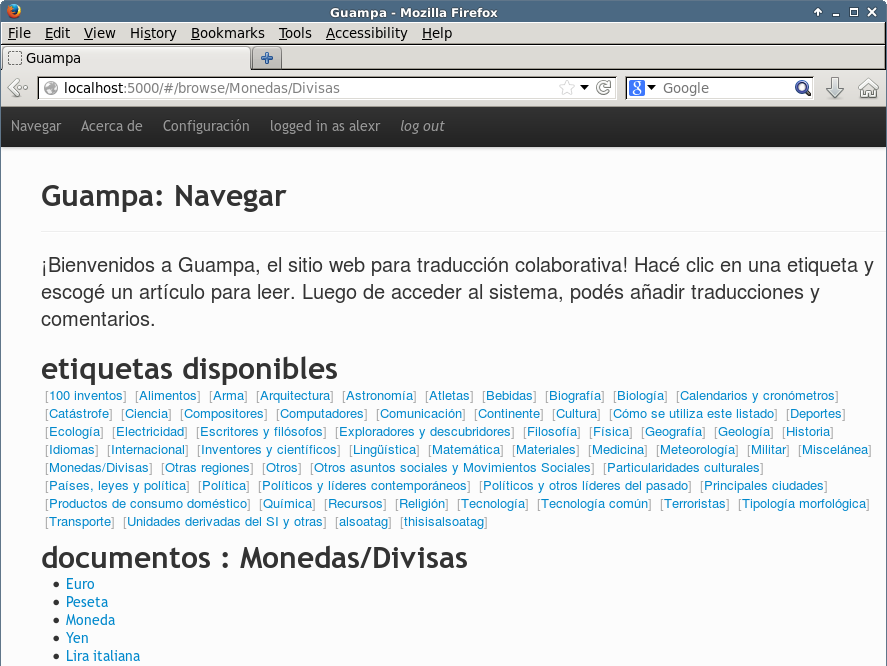
\includegraphics[width=12cm]{guampa-browse-cropped-updated}
  \end{center}
\caption{Screen shot of the interface for browsing documents. Here the
interface has been set to Paraguayan Spanish and the document database has been
populated with Spanish-language Wikipedia articles. Here we can browse articles
by tag.}
\label{fig:browse}
\end{figure*}

Tatoeba \cite{tatoeba} is a
project dedicated to collecting translations of sentences in many languages.
Users may add translations or correct the translations of other users by
providing alternate translations. However, genuine collaboration is not
facilitated since no history is available, and the focus is on the sentence
rather than the document. Traduwiki \cite{traduwiki} comes closer
to our goals; while it is intended for the collaborative translation of
documents, it is not open-source, and does not offer an easy way to export
training data for MT systems. In addition, development appears
to have stopped in 2007.

There have been a number of projects focused on using crowdsourcing to produce
bitext corpora for training MT systems. Notably, Ambati \emph{et al.}
\cite{ambati_naacl,ambati_act} have used active learning to construct a corpus
for training English-Spanish SMT, automatically creating Mechanical Turk tasks
to elicit translations for phrases that their system did not know how to
translate, but should. The Joshua team at Johns Hopkins has also successfully
used Mechanical Turk to crowdsource the creation of bitext corpora for SMT for
many languages of the Indian subcontinent
\cite{post-callisonburch-osborne:2012:WMT}. Both of these projects relied on a
populations of MTurk users familiar with the source and target languages.

Ambati \emph{et al.} \cite{Ambati:2012:CWC:2145204.2145382} have also described
another crowdsourcing approach that addresses the problem of finding bilingual
or nearly-bilingual crowd workers. In this work, they employ a multi-stage
process in which many ``weak bilinguals" (users somewhat skilled in both source
and target language, though not necessarily fluent) translate individual
lexical items, other turkers use these lexical items to construct candidate
translations, and then finally fluent speakers of the target language
synthesize sentences from these elements, without necessarily understanding the
source language.

These techniques, while exciting and applicable in many situations, may not be
applicable to all languages or language pairs. There are many parts of the
world in which Mechanical Turk is currently not broadly used, including most of
South America and Africa \cite{Pavlick-EtAl-2014:TACL}.  We posit that in these
cases, supporting an online community of translators may be more appropriate
than relying on one-off Mechanical Turk tasks.

\section{Guampa For Community Translation}
At its core, Guampa is a tool for translating documents. The central interface
of Guampa shows a document's source language text, segmented by sentence,
alongside the current translation for each sentence. For each sentence in the
document, users can add a new translation or edit the current translation.
This interface is shown in Figure \ref{fig:translating}.
The software stores the complete history of translation edits, along with
comments on the translation of a given sentence.

If a bilingual dictionary for the current language pair is present,
during editing, Guampa can present users with the relevant dictionary entries,
looking up each word in the current sentence and displaying possible lexical
translations underneath the editing interface. This process may be improved
with language-specific lemmatization to aid in dictionary lookups. Our
development version of Guampa includes a small Spanish-Guarani bilingual
dictionary and lemmatization for Spanish. This feature is enabled per-user, and
may easily be turned off on a settings page.

Users can discuss the best way to translate a particular passage and see the
history of the proposed translations for a sentence on a ``sentence history"
page, which is shown in Figure \ref{fig:history}.
Thus, Guampa is much like a wiki for translations; quality control is performed
through community consensus, and newer translators can learn from feedback.

Like the interface of Traduwiki, but in contrast to that of popular
internationalization tools like Pootle, our layout is intended to be suitable
for reading documents online. We intend it to be helpful for language learners
as well -- a user familiar with the source language and learning the target
language (or vice-versa) might benefit from reading translations side-by-side,
as in dual-language books.

\begin{figure*}
  \begin{center}
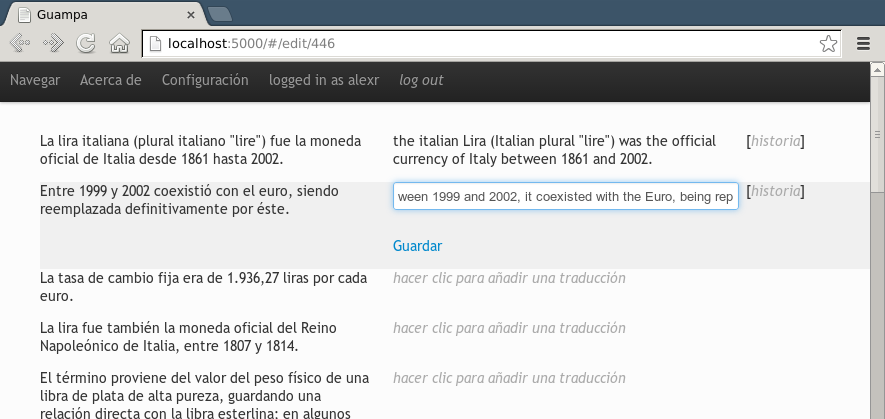
\includegraphics[width=12cm]{guampa-edit-cropped}
  \end{center}
\caption{Translating an article from the Spanish Wikipedia. From this screen,
we can edit the current translation for a sentence, or by clicking on the
history link, see the commentary and translations provided by other users.}
\label{fig:translating}
\end{figure*}

Users will normally select a document to read or translate on the navigation
interface, shown in Figure \ref{fig:browse}. Here one can browse the available
documents by tag.
Additional sorting criteria, such as recent activity and completeness of
translation, will be added soon.

Users must be logged in to add or edit translations, or to add comments.
Login is handled with Mozilla's Persona federated identity system,
\footnote{\url{http://login.persona.org/}}
which allows any user with an email address to log in.
Optionally, site operators may allow Guampa-specific accounts protected by
passwords.

For easy adaptability to different language pairs, the interface is built with
an internationalization package so that its strings can easily be replaced; our
development version has interfaces in Spanish and English, with Guarani coming
soon. Adding more languages as appropriate is straightforward, requiring very
few code changes. Additionally, the sentence segmenter for the source language
can easily be changed to locate sentence boundaries in different languages; our
development version uses the Punkt segmenter for Spanish from NLTK
\cite{nltkbook}.

\begin{figure*}
  \begin{center}
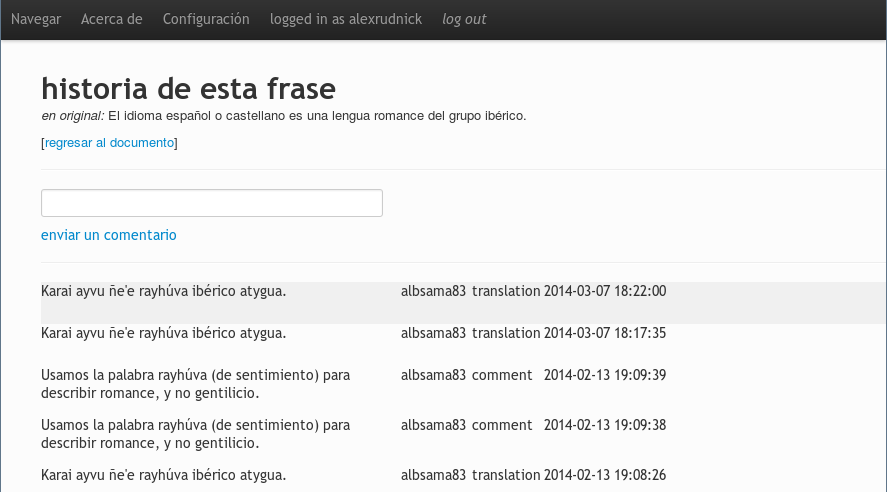
\includegraphics[width=12cm]{sentence-history-comment}
  \end{center}
\caption{The interface for the detailed history of a sentence; here users may
add new comments and see the translations that have been proposed for a given
sentence.}
\label{fig:history}
\end{figure*}

Guampa also features a simple interface for entering language-specific
diacritics, which may be difficult due to differences between available
keyboard layouts and the target language of the translations. Users may click
on buttons to add the appropriate diacritics, or can use a simple macro
language to type required characters; for example, the strings
\texttt{\string^a} or 
\texttt{\string~a} are automatically replaced with the nasalized `a',
\texttt{\~a}.
These features are currently specific to the Guarani language, but could easily
be adapted to other target languages.

\begin{figure}
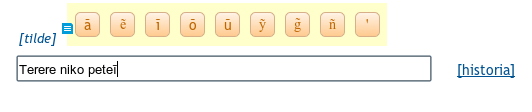
\includegraphics[width=8.25cm]{guampa-tildes}
\caption{Entering Guarani-language text with nasalized vowels. This screen shot
is from an early interface mockup; the deployed software may differ
somewhat.}
\label{fig:diacritics}
\end{figure}

\subsection{Guampa for Educational Use}
We are working in collaboration with Guarani institutions in Paraguay,
particularly the Ateneo de la Lengua Cultura Guarani
\footnote{\url{http://www.ateneoguarani.edu.py/}}
and the Fundación Yvy Mar\~{a}e'\~{y},
\footnote{\url{http://yvymaraey.org/}}
and the instructors at those institutions, to adapt the design of Guampa
so that it can be used in their translation courses, translation courses.
We want to enable collaborative translation and discussions among the students
and the instructor, both in the classroom and for homework assignments. This
will require allowing students to translate a single document independently,
without seeing each other's translations, a feature not implemented as of this
writing, but coming soon.

The instructor will be assigned a special role in the software, so that they
can see and moderate all translations entered by students. In the classroom,
the instructor will display the translations made by the students in order to
start a discussion on each of them.  Instructors will also be able to comment
on and rate each student translation and select their preferred translations
for each sentence, in order to produce a consensus translation for a given
document.

Some moderation and access control features will need to be added to support
this use case for Guampa; in general, different communities will have varying
norms and goals. Specifically, language style can be contentious, and
different communities may prefer different dialects and registers. In Paraguay,
for example, the extent to which Spanish loan-words are acceptable in written
Guarani is a divisive issue, so the users of a given Guampa installation will
need to address this on their own. Analogous considerations will be relevant
for many language communities.

\subsection{Importing Documents, Exporting Bitext}
For populating a new instance of Guampa, we include scripts to extract
plain-text versions of Wikipedia articles from Wikipedia database dumps
\footnote{Complete copies of Wikipedias can be downloaded at \\
\url{http://dumps.wikimedia.org/}}, providing source-language documents for a
new installation of Guampa. Our tools build on the Wikipedia Extractor
script from the Medialab at the University of Pisa \cite{pisa-wp-extractor}.

However, for some source languages, such as English or Spanish, importing an
entire Wikipedia would overwhelm both the server and the users. Fortunately,
many Wikipedias include a list of so-called ``vital articles", subjects for
which it is felt that high-quality articles are essential in any encyclopedia.
These lists typically contain roughly one thousand articles. We provide scripts
to extract and import only these articles, and to tag them with their
appropriate subcategories (such as ``Science" or ``Biography"), which are
automatically extracted from the list structure of the document.

For some language pairs and user communities, it may be appropriate to import
an entire Wikipedia into Guampa\footnote{
For example, as of this writing there are fewer than three thousand
articles in the Guarani Wikipedia.}
for translation into another language. This approach is also supported.

Documents from other sources can also be imported into Guampa for translation;
PDF, ODF, and Microsoft Word documents can be imported with the use of scripts
that rely on Apache Tika\footnote{\url{http://tika.apache.org/}}
to convert them into plain text. Users will have
access to this functionality through the web interface in the near future.

Guampa also includes a script for easy export of bitext sentences; since the
system keeps an internal representation of sentence boundaries in the original
documents, it is easy to export one sentence per line into the output files. To
train an MT system, one would then run the appropriate preprocessing and
training pipeline on these exported files. In the near term, we also plan to
add export features in HTML and MediaWiki markup, for ease of publishing the
translated documents and adding them to the target-language Wikipedia.

\section{Implementation}
Guampa is a web application, with a user interface made of the AngularJS
\cite{angularjs} and Bootstrap \cite{bootstrap} toolkits. We internationalize
the user interface with the angular-translate package \cite{angular-translate}.
The server side of the application is implemented in Python 3, using the Flask
micro-framework \cite{flask}, SQLAlchemy
\cite{sqlalchemy} for object-relational mapping, and SQLite \cite{sqlite} as a
database. SQLite could easily be replaced with a more industrial-scale
database, should the need arise.

Guampa is straightforward to install in production and is known to work well
with the Apache web server on Ubuntu Linux, though other UNIX-like systems and
WSGI-capable servers should also work. For development work, scripts are
provided to set up the required environment (with virtualenv) and to run a
development server; these are known to work well on both Linux and Mac OS X.

\section{Conclusions and Future Work}
Here we have described Guampa, a free software tool for collaborative online
translation.
In collaboration with language educators, learners, and activists in Paraguay,
we will use Guampa to build bitext corpora for Spanish-Guarani for our
continuing MT work with that language pair. These resources will be made
publicly available on our website, along with Guampa and our other software.
We will also adapt Guampa for educational use in Guarani-language classes.

As we continue development of Guampa, with feedback and suggestions from our
users, we plan to add additional features, including recognition for prolific
translators, similar to Wikipedia's Barnstars. We would like to develop other
features to help users encourage themselves, including a feature to send
periodic translation tasks by email, so that users can be reminded to practice
daily. Additionally, we will implement exporting over the web and into formats
other than plain text -- such as TMX, Mediawiki markup, and HTML --  to
facilitate reuse of the collected corpora for reading, for MT-related uses, and
for integration into the target-language Wikipedias.

More technically ambitious and longer-range future features will include lookup
in a translation memory, with pluggable morphological analysis, and integrated
suggestions from machine translation. Our long-term goal is for Guampa to
become a full-fledged collaborative computer-assisted translation tool.

Guampa is released under the GPLv3 and available on GitHub at:
\\
\url{http://github.com/hltdi/guampa} , with a live demo server linked from that
site. It is under active development but is already relatively easy to install
and adapt to the particularities of different language pairs and the needs of
different translation communities. We welcome suggestions, bug reports,
questions, doubts, and development collaborators!

\bibliographystyle{lrec2014}
\bibliography{guampa}

\end{document}
